\section{Driving Smoothness}
\label{sec:Results_Smoothness}

The driving smoothness analysis examines the average acceleration $\gls{a}$ and jerk $\gls{j}$ as functions of the \ac{mpr} of equipped vehicles. Table~\ref{tab:DrivingSmoothness} reports the paired values $(\gls{a},\gls{j})$ for the Standard, \ac{flow-glosa}, and \ac{eco-glosa} configurations under both the HBEFA4 and PHEMlight5 models. Figures~\ref{fig:Smoothness_692}, \ref{fig:Smoothness_2769}, and \ref{fig:Smoothness_3462} illustrate these trends at representative traffic volumes of $692$, $2769$, and $3462\,\mathrm{veh/h}$.

\paragraph{\ac{eco-glosa} at low to medium volumes}
Under \ac{eco-glosa}, as \ac{mpr} increases from $0\%$ to $100\%$, the average acceleration decreases while jerk increases. For example, at $69\,\mathrm{veh/h}$ with HBEFA4, acceleration falls from $0.30\,\mathrm{m/s^2}$ to $0.25\,\mathrm{m/s^2}$ (a $17\%$ reduction), whereas jerk rises from $0.74\,\mathrm{m/s^3}$ to $0.81\,\mathrm{m/s^3}$ (a $9\%$ increase). A similar pattern occurs under PHEMlight5: acceleration decreases from $0.30$ to $0.23\,\mathrm{m/s^2}$, and jerk increases from $0.74$ to $0.81\,\mathrm{m/s^3}$ (Table~\ref{tab:DrivingSmoothness}). At $692\,\mathrm{veh/h}$, HBEFA4 acceleration drops from $0.32$ to $0.26\,\mathrm{m/s^2}$ and jerk increases from $0.74$ to $0.80\,\mathrm{m/s^3}$ (Fig.~\ref{fig:Smoothness_HBEFA4_692}). Under PHEMlight5, the pattern is analogous (Fig.~\ref{fig:Smoothness_PHEMlight5_692}). This reflects vehicles adjusting speed to exploit green-wave opportunities, resulting in gentler accelerations ($\Delta a<0$) but sharper decelerations when gaps are encountered ($\Delta j>0$).

\paragraph{\ac{eco-glosa} at high volume ($2769\,\mathrm{veh/h}$)}
At $2769\,\mathrm{veh/h}$, HBEFA4 acceleration under \ac{eco-glosa} fluctuates around the Standard: it increases from $0.36$ at $0\%$ to $0.41\,\mathrm{m/s^2}$ at $30\%$ MPR, then decreases toward $0.27\,\mathrm{m/s^2}$ at full penetration (Fig.~\ref{fig:Smoothness_HBEFA4_2769}). Jerk similarly oscillates, reflecting intermittent congestion relief. Under PHEMlight5, however, acceleration steadily improves from $0.36$ to $0.33\,\mathrm{m/s^2}$, and jerk increases to a maximum of $0.59\,\mathrm{m/s^3}$ at $30\%$ then declines to $0.66\,\mathrm{m/s^3}$ at $100\%$, still $13\%$ below the Standard value of $0.76\,\mathrm{m/s^3}$ (Fig.~\ref{fig:Smoothness_PHEMlight5_2769}). The persistently lower jerk at high MPR suggests that, once the existing jam is traversed, vehicles maintain smoother trajectories even as they accelerate less aggressively.

\paragraph{\ac{eco-glosa} at full saturation ($3462\,\mathrm{veh/h}$)}
In the fully saturated regime, both models exhibit monotonic smoothness improvements. For HBEFA4, acceleration decreases from $0.55$ to $0.38\,\mathrm{m/s^2}$ (a $31\%$ reduction) and jerk from $0.57$ to $0.51\,\mathrm{m/s^3}$ (an $11\%$ reduction) as \ac{mpr} rises from $0\%$ to $100\%$ (Fig.~\ref{fig:Smoothness_HBEFA4_3462}). PHEMlight5 shows comparable gains, with acceleration falling from $0.55$ to $0.35\,\mathrm{m/s^2}$ and jerk from $0.57$ to $0.52\,\mathrm{m/s^3}$ (Fig.~\ref{fig:Smoothness_PHEMlight5_3462}). These results indicate that, beyond the capacity limit, equipped vehicles coordinate to reduce stop‐and‐go oscillations, yielding continuously smoother motion.

\paragraph{\ac{flow-glosa} comparison}
Across all volumes, \ac{flow-glosa} offers acceleration improvements comparable to \ac{eco-glosa} but consistently lower jerk. At low to medium volumes, acceleration under \ac{flow-glosa} decreases by approximately $15$–$20\%$ from the Standard, while jerk increases by only $5$–$8\%$, remaining below \ac{eco-glosa} values (Table~\ref{tab:DrivingSmoothness}). At full saturation ($3462\,\mathrm{veh/h}$), \ac{flow-glosa} exhibits a notable jerk spike from $0.59$ to $0.71\,\mathrm{m/s^3}$ at $\mathrm{MPR}=60\%$, corresponding to the point at which the existing jam dissolves and vehicles resume free‐flow conditions. At \ac{mpr} of $80\%$, the pronounced jerk peak does not stem from an incoming traffic jam but from platoon‐based micro-adjustments. With such a high share of equipped vehicles, tight vehicle clusters form and must continually realign to the signal phases. Minor mismatches force abrupt decelerations when a platoon splits or catches a red, followed by rapid accelerations to reform the cluster. These frequent, short-interval speed changes drive the observed transient increase in jerk.

\begin{figure}[htb]
  \centering
  \begin{subfigure}[b]{0.45\textwidth}
    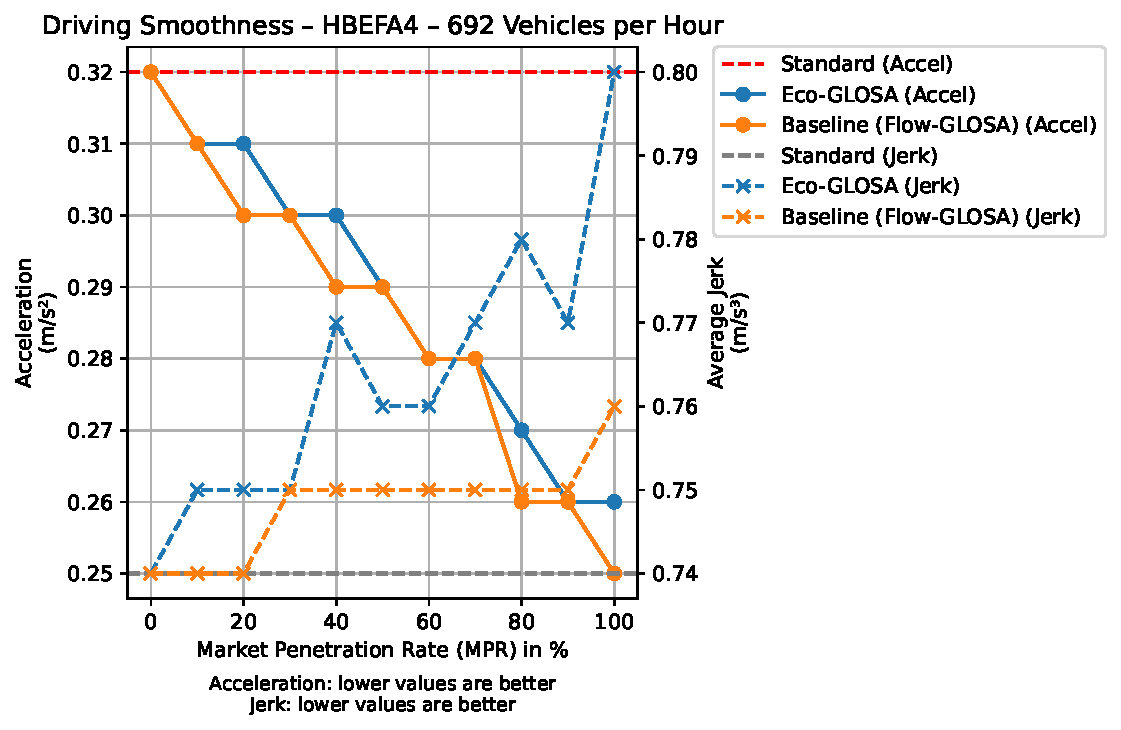
\includegraphics[width=\textwidth]{data/img/DrivingSmoothness/DrivingSmoothness_HBEFA4_Cars692.pdf}
    \caption{Average acceleration and jerk versus \ac{mpr} for HBEFA4 at $692\,\mathrm{veh/h}$.}
    \label{fig:Smoothness_HBEFA4_692}
  \end{subfigure}\hfill
  \begin{subfigure}[b]{0.45\textwidth}
    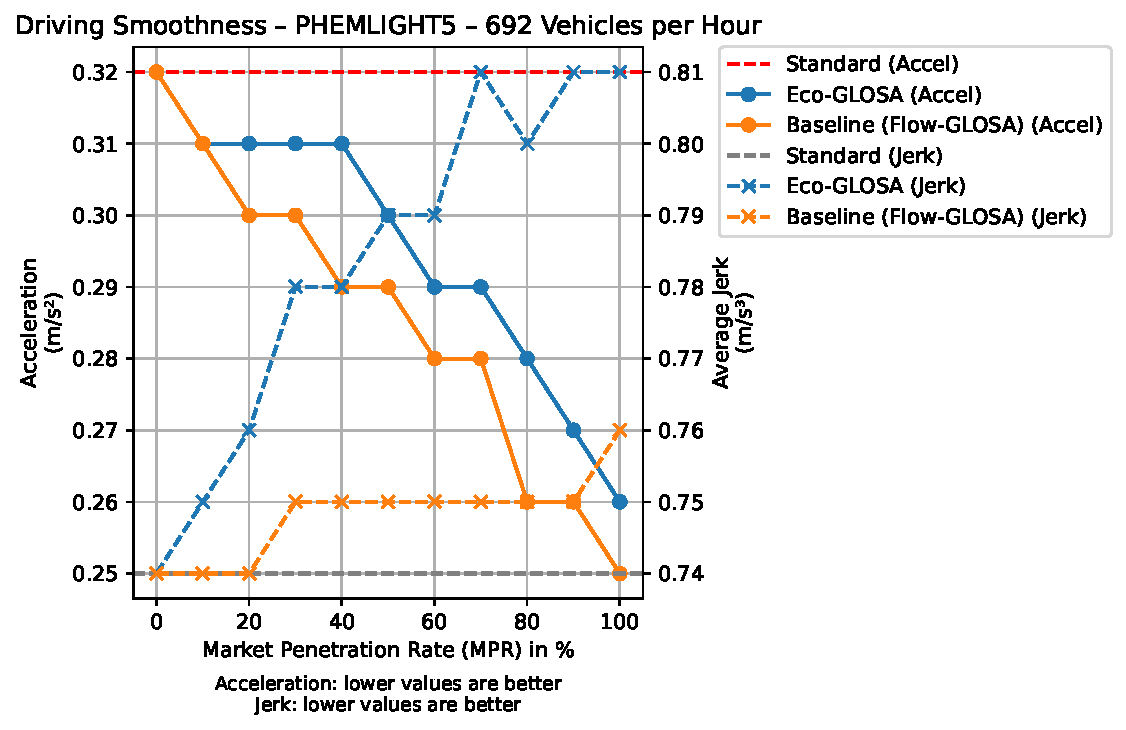
\includegraphics[width=\textwidth]{data/img/DrivingSmoothness/DrivingSmoothness_PHEMLIGHT5_Cars692.pdf}
    \caption{Average acceleration and jerk versus \ac{mpr} for PHEMlight5 at $692\,\mathrm{veh/h}$.}
    \label{fig:Smoothness_PHEMlight5_692}
  \end{subfigure}
  \caption{Driving smoothness as a function of \ac{mpr} at $692\,\mathrm{veh/h}$, comparing Standard, \ac{eco-glosa}, and \ac{flow-glosa}.}
  \label{fig:Smoothness_692}
\end{figure}

\begin{figure}[htb]
  \centering
  \begin{subfigure}[b]{0.45\textwidth}
    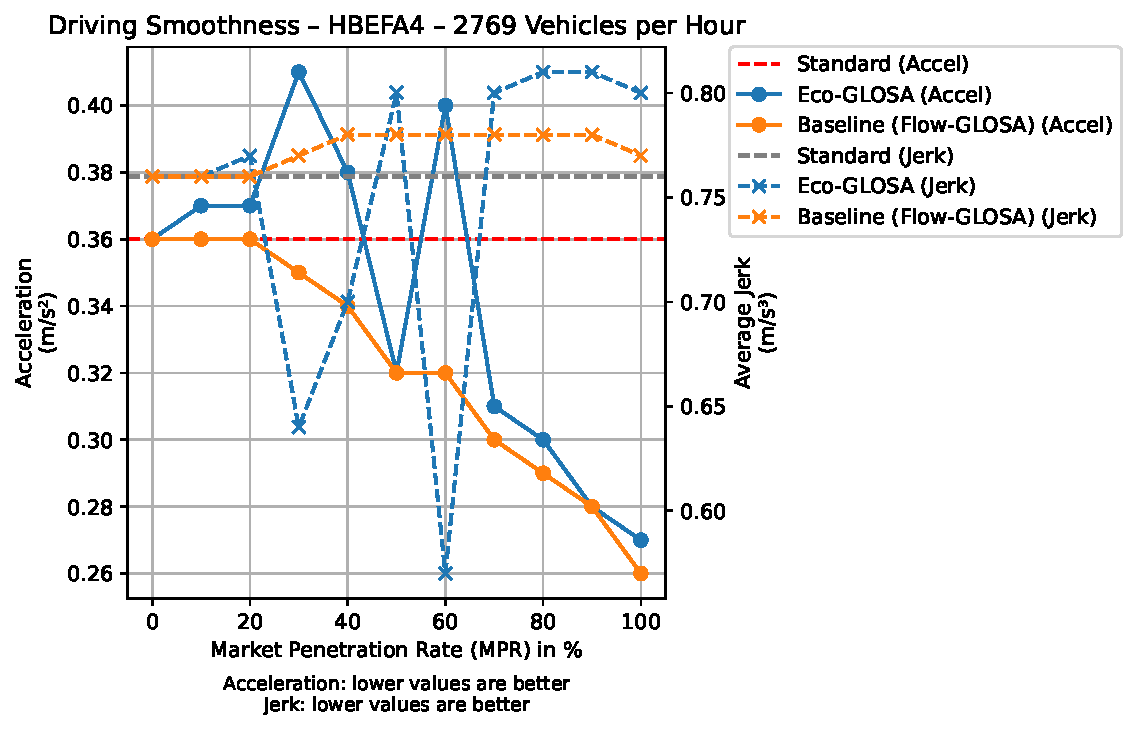
\includegraphics[width=\textwidth]{data/img/DrivingSmoothness/DrivingSmoothness_HBEFA4_Cars2769.pdf}
    \caption{Average acceleration and jerk versus \ac{mpr} for HBEFA4 at $2769\,\mathrm{veh/h}$.}
    \label{fig:Smoothness_HBEFA4_2769}
  \end{subfigure}\hfill
  \begin{subfigure}[b]{0.45\textwidth}
    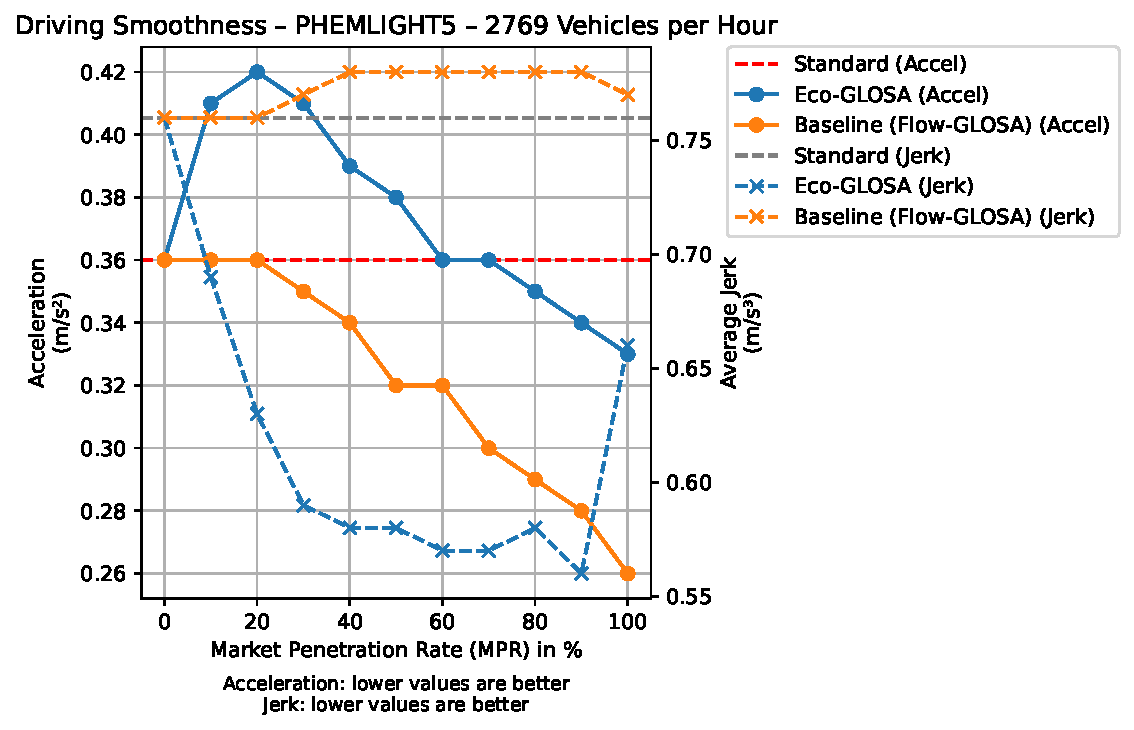
\includegraphics[width=\textwidth]{data/img/DrivingSmoothness/DrivingSmoothness_PHEMLIGHT5_Cars2769.pdf}
    \caption{Average acceleration and jerk versus \ac{mpr} for PHEMlight5 at $2769\,\mathrm{veh/h}$.}
    \label{fig:Smoothness_PHEMlight5_2769}
  \end{subfigure}
  \caption{Driving smoothness as a function of \ac{mpr} at $2769\,\mathrm{veh/h}$, comparing Standard, \ac{eco-glosa}, and \ac{flow-glosa}.}
  \label{fig:Smoothness_2769}
\end{figure}

\begin{figure}[htb]
  \centering
  \begin{subfigure}[b]{0.45\textwidth}
    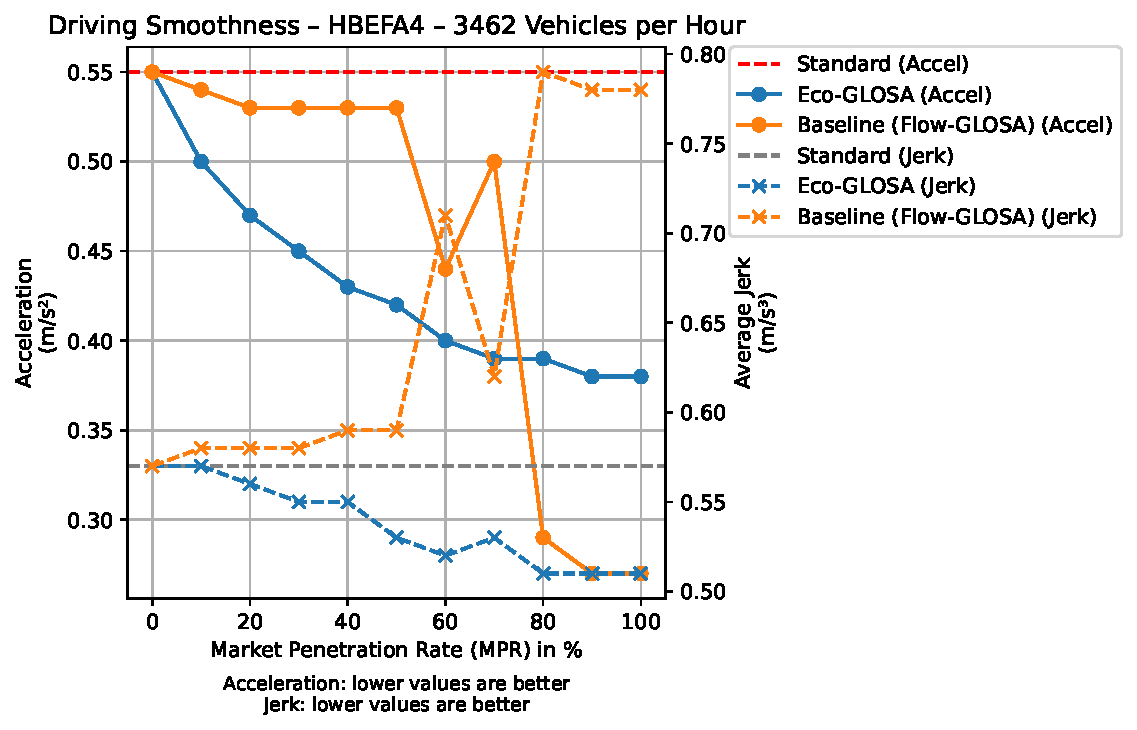
\includegraphics[width=\textwidth]{data/img/DrivingSmoothness/DrivingSmoothness_HBEFA4_Cars3462.pdf}
    \caption{Average acceleration and jerk versus \ac{mpr} for HBEFA4 at $3462\,\mathrm{veh/h}$.}
    \label{fig:Smoothness_HBEFA4_3462}
  \end{subfigure}\hfill
  \begin{subfigure}[b]{0.45\textwidth}
    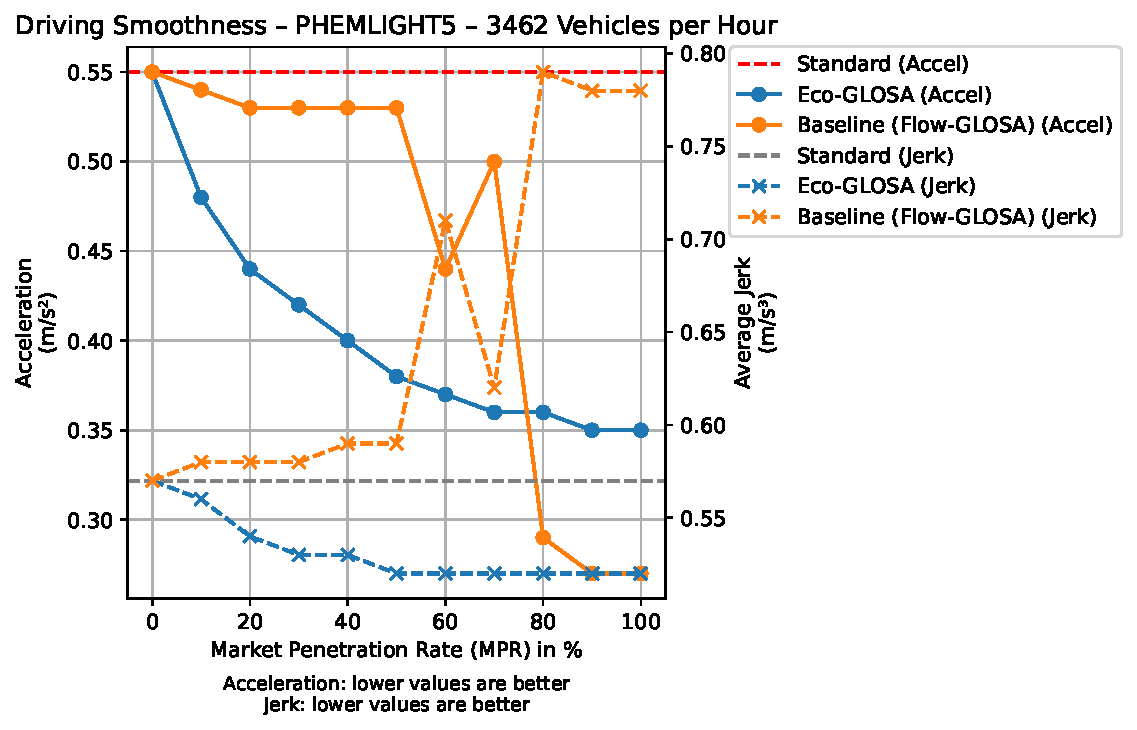
\includegraphics[width=\textwidth]{data/img/DrivingSmoothness/DrivingSmoothness_PHEMLIGHT5_Cars3462.pdf}
    \caption{Average acceleration and jerk versus \ac{mpr} for PHEMlight5 at $3462\,\mathrm{veh/h}$.}
    \label{fig:Smoothness_PHEMlight5_3462}
  \end{subfigure}
  \caption{Driving smoothness as a function of \ac{mpr} at $3462\,\mathrm{veh/h}$, comparing Standard, \ac{eco-glosa}, and \ac{flow-glosa}.}
  \label{fig:Smoothness_3462}
\end{figure}

\begin{table}[htb]
  \centering
  \caption{Driving smoothness in terms of average acceleration (m/s\textsuperscript{2}) and jerk (m/s\textsuperscript{3}) for various traffic volumes and \acp{mpr}. Results are provided for the Standard (no \ac{glosa}), \ac{flow-glosa}, and \ac{eco-glosa} configurations under the HBEFA4 and PHEMlight5 emission models.}
  \label{tab:DrivingSmoothness}
  \resizebox{\textwidth}{!}{%
    \begin{tabular}{l l l *{11}{c}}
      \toprule
      Cars & Algorithm & Model       & \textbf{0\% (Standard)} & 10\%        & 20\%        & 30\%        & 40\%        & 50\%        & 60\%        & 70\%        & 80\%        & 90\%        & 100\%       \\
      \midrule
      \textbf{69.0}  & Eco-GLOSA                   & HBEFA4      & \textbf{0.3, 0.74}   & 0.29, 0.75  & 0.31, 0.76  & 0.28, 0.77  & 0.29, 0.77  & 0.29, 0.79  & 0.27, 0.77  & 0.25, 0.81  & 0.28, 0.80  & 0.24, 0.79  & 0.25, 0.81  \\
      \textbf{69.0}  & Baseline (Flow-GLOSA)       & HBEFA4      & \textbf{0.3, 0.74}   & 0.29, 0.76  & 0.31, 0.75  & 0.28, 0.75  & 0.28, 0.75  & 0.29, 0.75  & 0.28, 0.74  & 0.25, 0.75  & 0.27, 0.75  & 0.25, 0.75  & 0.25, 0.77  \\
      \textbf{69.0}  & Eco-GLOSA                   & PHEMlight5  & \textbf{0.3, 0.74}   & 0.29, 0.76  & 0.29, 0.75  & 0.28, 0.76  & 0.27, 0.78  & 0.28, 0.78  & 0.27, 0.80  & 0.25, 0.81  & 0.27, 0.80  & 0.24, 0.79  & 0.23, 0.81  \\
      \textbf{69.0}  & Baseline (Flow-GLOSA)       & PHEMlight5  & \textbf{0.3, 0.74}   & 0.29, 0.76  & 0.31, 0.75  & 0.28, 0.75  & 0.28, 0.75  & 0.29, 0.75  & 0.28, 0.74  & 0.25, 0.75  & 0.27, 0.75  & 0.25, 0.75  & 0.25, 0.77  \\
      \midrule
      \textbf{138.0} & Eco-GLOSA                   & HBEFA4      & \textbf{0.31, 0.73}  & 0.29, 0.74  & 0.30, 0.74  & 0.28, 0.74  & 0.28, 0.77  & 0.27, 0.76  & 0.28, 0.77  & 0.25, 0.77  & 0.27, 0.78  & 0.26, 0.79  & 0.25, 0.78  \\
      \textbf{138.0} & Baseline (Flow-GLOSA)       & HBEFA4      & \textbf{0.31, 0.73}  & 0.29, 0.74  & 0.30, 0.75  & 0.30, 0.73  & 0.28, 0.75  & 0.28, 0.74  & 0.27, 0.75  & 0.26, 0.74  & 0.27, 0.75  & 0.26, 0.74  & 0.25, 0.75  \\
      \textbf{138.0} & Eco-GLOSA                   & PHEMlight5  & \textbf{0.31, 0.73}  & 0.30, 0.73  & 0.29, 0.75  & 0.28, 0.75  & 0.28, 0.77  & 0.26, 0.76  & 0.26, 0.78  & 0.26, 0.77  & 0.26, 0.79  & 0.25, 0.79  & 0.24, 0.79  \\
      \textbf{138.0} & Baseline (Flow-GLOSA)       & PHEMlight5  & \textbf{0.31, 0.73}  & 0.29, 0.74  & 0.30, 0.75  & 0.30, 0.73  & 0.28, 0.75  & 0.28, 0.74  & 0.27, 0.75  & 0.26, 0.74  & 0.27, 0.75  & 0.26, 0.74  & 0.25, 0.75  \\
      \midrule
      \textbf{346.0} & Eco-GLOSA                   & HBEFA4      & \textbf{0.31, 0.74}  & 0.31, 0.75  & 0.31, 0.76  & 0.30, 0.76  & 0.29, 0.76  & 0.29, 0.77  & 0.28, 0.77  & 0.28, 0.77  & 0.27, 0.77  & 0.26, 0.79  & 0.25, 0.80  \\
      \textbf{346.0} & Baseline (Flow-GLOSA)       & HBEFA4      & \textbf{0.31, 0.74}  & 0.31, 0.76  & 0.30, 0.75  & 0.30, 0.76  & 0.29, 0.76  & 0.29, 0.76  & 0.27, 0.75  & 0.28, 0.75  & 0.26, 0.76  & 0.26, 0.76  & 0.24, 0.76  \\
      \textbf{346.0} & Eco-GLOSA                   & PHEMlight5  & \textbf{0.31, 0.74}  & 0.31, 0.75  & 0.31, 0.77  & 0.30, 0.77  & 0.29, 0.77  & 0.28, 0.80  & 0.28, 0.79  & 0.28, 0.78  & 0.26, 0.79  & 0.26, 0.80  & 0.25, 0.82  \\
      \textbf{346.0} & Baseline (Flow-GLOSA)       & PHEMlight5  & \textbf{0.31, 0.74}  & 0.31, 0.76  & 0.30, 0.75  & 0.30, 0.76  & 0.29, 0.76  & 0.29, 0.76  & 0.27, 0.75  & 0.28, 0.75  & 0.26, 0.76  & 0.26, 0.76  & 0.24, 0.76  \\
      \midrule
      \textbf{692.0} & Eco-GLOSA                   & HBEFA4      & \textbf{0.32, 0.74}  & 0.31, 0.75  & 0.31, 0.75  & 0.30, 0.75  & 0.30, 0.77  & 0.29, 0.76  & 0.28, 0.76  & 0.28, 0.77  & 0.27, 0.78  & 0.26, 0.77  & 0.26, 0.80  \\
      \textbf{692.0} & Baseline (Flow-GLOSA)       & HBEFA4      & \textbf{0.32, 0.74}  & 0.31, 0.74  & 0.30, 0.74  & 0.30, 0.75  & 0.29, 0.75  & 0.29, 0.75  & 0.28, 0.75  & 0.28, 0.75  & 0.26, 0.75  & 0.26, 0.75  & 0.25, 0.76  \\
      \textbf{692.0} & Eco-GLOSA                   & PHEMlight5  & \textbf{0.32, 0.74}  & 0.31, 0.75  & 0.31, 0.76  & 0.31, 0.78  & 0.31, 0.78  & 0.30, 0.79  & 0.29, 0.79  & 0.29, 0.81  & 0.28, 0.80  & 0.27, 0.81  & 0.26, 0.81  \\
      \textbf{692.0} & Baseline (Flow-GLOSA)       & PHEMlight5  & \textbf{0.32, 0.74}  & 0.31, 0.74  & 0.30, 0.74  & 0.30, 0.75  & 0.29, 0.75  & 0.29, 0.75  & 0.28, 0.75  & 0.28, 0.75  & 0.26, 0.75  & 0.26, 0.75  & 0.25, 0.76  \\
      \midrule
      \textbf{1385.0}& Eco-GLOSA                   & HBEFA4      & \textbf{0.33, 0.74}  & 0.33, 0.75  & 0.33, 0.76  & 0.32, 0.77  & 0.31, 0.77  & 0.31, 0.77  & 0.30, 0.78  & 0.29, 0.78  & 0.28, 0.78  & 0.27, 0.78  & 0.26, 0.78  \\
      \textbf{1385.0}& Baseline (Flow-GLOSA)       & HBEFA4      & \textbf{0.33, 0.74}  & 0.33, 0.75  & 0.33, 0.75  & 0.32, 0.76  & 0.31, 0.76  & 0.30, 0.76  & 0.29, 0.76  & 0.29, 0.76  & 0.27, 0.76  & 0.27, 0.76  & 0.26, 0.75  \\
      \textbf{1385.0}& Eco-GLOSA                   & PHEMlight5  & \textbf{0.33, 0.74}  & 0.34, 0.77  & 0.34, 0.79  & 0.34, 0.80  & 0.33, 0.81  & 0.32, 0.82  & 0.32, 0.84  & 0.30, 0.83  & 0.29, 0.83  & 0.28, 0.84  & 0.27, 0.83  \\
      \textbf{1385.0}& Baseline (Flow-GLOSA)       & PHEMlight5  & \textbf{0.33, 0.74}  & 0.33, 0.75  & 0.33, 0.75  & 0.32, 0.76  & 0.31, 0.76  & 0.30, 0.76  & 0.29, 0.76  & 0.29, 0.76  & 0.27, 0.76  & 0.27, 0.76  & 0.26, 0.75  \\
      \midrule
      \textbf{2077.0}& Eco-GLOSA                   & HBEFA4      & \textbf{0.34, 0.75}  & 0.34, 0.75  & 0.35, 0.76  & 0.34, 0.77  & 0.33, 0.78  & 0.32, 0.78  & 0.31, 0.78  & 0.30, 0.79  & 0.29, 0.79  & 0.28, 0.78  & 0.27, 0.78  \\
      \textbf{2077.0}& Baseline (Flow-GLOSA)       & HBEFA4      & \textbf{0.34, 0.75}  & 0.34, 0.76  & 0.34, 0.76  & 0.33, 0.76  & 0.32, 0.77  & 0.32, 0.77  & 0.30, 0.77  & 0.29, 0.77  & 0.28, 0.76  & 0.26, 0.76  & 0.26, 0.76  \\
      \textbf{2077.0}& Eco-GLOSA                   & PHEMlight5  & \textbf{0.34, 0.75}  & 0.36, 0.78  & 0.35, 0.80  & 0.35, 0.82  & 0.34, 0.84  & 0.32, 0.84  & 0.31, 0.85  & 0.31, 0.87  & 0.29, 0.86  & 0.28, 0.86  & 0.27, 0.87  \\
      \textbf{2077.0}& Baseline (Flow-GLOSA)       & PHEMlight5  & \textbf{0.34, 0.75}  & 0.34, 0.76  & 0.34, 0.76  & 0.33, 0.76  & 0.32, 0.77  & 0.32, 0.77  & 0.30, 0.77  & 0.29, 0.77  & 0.28, 0.76  & 0.26, 0.76  & 0.26, 0.76  \\
      \midrule
      \textbf{2769.0}& Eco-GLOSA                   & HBEFA4      & \textbf{0.36, 0.76}  & 0.37, 0.76  & 0.37, 0.77  & 0.41, 0.64  & 0.38, 0.70  & 0.32, 0.80  & 0.40, 0.57  & 0.31, 0.80  & 0.30, 0.81  & 0.28, 0.81  & 0.27, 0.80  \\
      \textbf{2769.0}& Baseline (Flow-GLOSA)       & HBEFA4      & \textbf{0.36, 0.76}  & 0.36, 0.76  & 0.36, 0.76  & 0.35, 0.77  & 0.34, 0.78  & 0.32, 0.78  & 0.32, 0.78  & 0.30, 0.78  & 0.29, 0.78  & 0.28, 0.78  & 0.26, 0.77  \\
      \textbf{2769.0}& Eco-GLOSA                   & PHEMlight5  & \textbf{0.36, 0.76}  & 0.41, 0.69  & 0.42, 0.63  & 0.41, 0.59  & 0.39, 0.58  & 0.38, 0.58  & 0.36, 0.57  & 0.36, 0.57  & 0.35, 0.58  & 0.34, 0.56  & 0.33, 0.66  \\
      \textbf{2769.0}& Baseline (Flow-GLOSA)       & PHEMlight5  & \textbf{0.36, 0.76}  & 0.36, 0.76  & 0.36, 0.76  & 0.35, 0.77  & 0.34, 0.78  & 0.32, 0.78  & 0.32, 0.78  & 0.30, 0.78  & 0.29, 0.78  & 0.28, 0.78  & 0.26, 0.77  \\
      \midrule
      \textbf{3462.0} & \textbf{Eco-GLOSA} & \textbf{HBEFA4} & \textbf{0.55, 0.57} & \textbf{0.50, 0.57} & \textbf{0.47, 0.56} & \textbf{0.45, 0.55} & \textbf{0.43, 0.55} & \textbf{0.42, 0.53} & \textbf{0.40, 0.52} & \textbf{0.39, 0.53} & \textbf{0.39, 0.51} & \textbf{0.38, 0.51} & \textbf{0.38, 0.51} \\
      \textbf{3462.0}& Baseline (Flow-GLOSA)       & HBEFA4      & \textbf{0.55, 0.57}  & 0.54, 0.58  & 0.53, 0.58  & 0.53, 0.58  & 0.53, 0.59  & 0.53, 0.59  & 0.44, 0.71  & 0.50, 0.62  & \textbf{0.29, 0.79}  & \textbf{0.27, 0.78}  & \textbf{0.27, 0.78}  \\
      \textbf{3462.0} & \textbf{Eco-GLOSA} & \textbf{PHEMlight5} & \textbf{0.55, 0.57} & \textbf{0.48, 0.56} & \textbf{0.44, 0.54} & \textbf{0.42, 0.53} & \textbf{0.40, 0.53} & \textbf{0.38, 0.52} & \textbf{0.37, 0.52} & \textbf{0.36, 0.52} & \textbf{0.36, 0.52} & \textbf{0.35, 0.52} & \textbf{0.35, 0.52} \\
      \textbf{3462.0}& Baseline (Flow-GLOSA)       & PHEMlight5  & \textbf{0.55, 0.57}  & 0.54, 0.58  & 0.53, 0.58  & 0.53, 0.58  & 0.53, 0.59  & 0.53, 0.59  & 0.44, 0.71  & 0.50, 0.62  & \textbf{0.29, 0.79}  & \textbf{0.27, 0.78}  & \textbf{0.27, 0.78}  \\
      \bottomrule
    \end{tabular}%
  }
\end{table}
